
\section{Generating Open-Ended Forecasting Questions from News}
\label{sec:questions_data}

\looseness -1 We now discuss our methodology to convert daily news articles into forecasting questions using language models. Any fixed forecasting dataset loses value as newer base models with training cutoffs after the dataset was created are adopted. Thus, we first describe the general methodology which can be used in the future, and then describe the specific instantiations we used to create our training data \ourdataset which has questions until April 2025. We conclude by demonstrating forecasting improvements due to our data filtering steps.

\subsection{Methodology for Generating Forecasting Questions}
\label{sec:question_creation_pipeline}

\begin{figure}[t]
\vspace{-0.6cm}
    \centering
    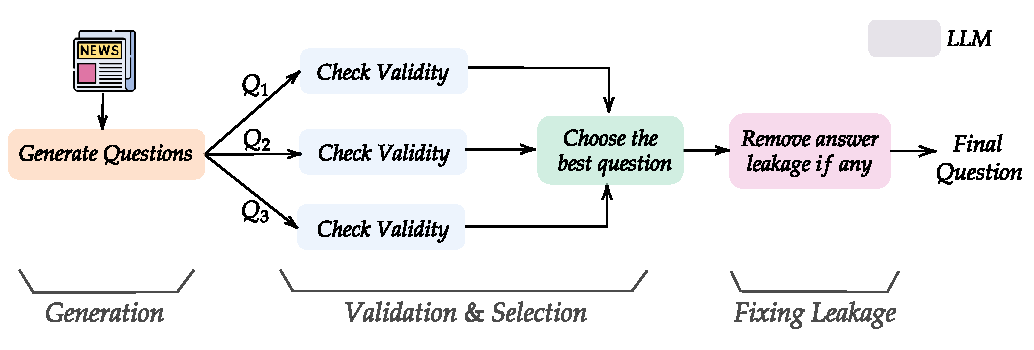
\includegraphics[width=0.885\textwidth]{figures/qgen/qgen_pipeline3.pdf}
    \vspace{-0.3cm} 
    \caption{\textbf{Our question generation methodology.} We use DeepSeek-v3 to generate multiple forecasting questions per news article. Then, we use Llama-4-Maverick to check if questions follow all guidelines, choose the best question, and remove any hints revealing the answer.}
    \label{fig:qgen_pipeline}
    \vspace{-0.4cm} 
\end{figure}

We generate short-answer, open-ended forecasting questions from individual news articles as illustrated in \Cref{fig:qgen_pipeline}. We describe each step in detail below:

\textbf{Sourcing Event Information.}
News outlets establish global infrastructure for reporting salient events as they occur. Unfortunately, \citet{paleka2025pitfalls} show that sourcing news via online search engines is unreliable. While search engines provide date cutoffs, future information can leak through updates to articles after the publish date, and even search engine ranking. This compromises the reliablity of backtests, and leaks future information in training, which can hurt Deep Learning models that easily overfit to spurious correlations. Fortunately, the CommonCrawl News (CCNews) Corpus~\citep{nagel2016-ccnews} provides static monthly snapshots of global news with accurate dates. This makes it free and easy to obtain news articles for creating forecasting questions. \vspace{0.15cm}


\textbf{Generating samples from documents.} Based on each news article, we ask a \textit{sample creator} model to generate up to three diverse forecasting samples. Each sample consists of: 
\begin{enumerate}
    \item \textbf{Question:} Asks about the prediction of an event. %, often with an explicit deadline (e.g., ``by \textit{Month, Year}'').
    \item \textbf{Background:} Provides brief context, and defines uncommon terms.
    \item \textbf{Resolution criteria:} Fixes a source of truth, proposes a resolution date for the question, and the expected answer format.
    \item \textbf{Answer:} Drawn verbatim from the article, unique, short (usually 1–3 words), and non-numeric (usually a name or location).
    \item \textbf{Source article link:} Obtained from article metadata for future reference.
\end{enumerate} \vspace{0.15cm}

\begin{tcolorbox}[title=\textbf{Sample Generated Forecasting Question}, colframe=black!70, colback=black!2, boxrule=0.5pt, breakable]
\textbf{Question.} Who will be confirmed as the new prime minister of Ukraine by 17 July 2025?

\medskip
\textbf{Background.}
Ukraine's parliament is scheduled to vote to appoint a new prime minister.

\medskip
\textbf{Resolution Criteria.}
\begin{itemize}[leftmargin=1.1em, itemsep=0.2em]
  \item \textbf{Source of Truth:} Official announcement from the Verkhovna Rada (Ukraine's parliament) confirming the appointment, via parliamentary records or government press release.
  \item \textbf{Resolution Date:} 17 July 2025, the date on which the parliamentary vote occurs and results are published.
  \item \textbf{Accepted Answer Format:} Full name of the individual exactly as given in the parliamentary announcement.
\end{itemize}

\medskip
\textbf{Answer Type.} String (Name)

\medskip
\textbf{Ground-Truth Answer.} Yulia Svyrydenko

\medskip
\textbf{Source.} The Guardian (live blog): \href{https://www.theguardian.com/world/live/2025/jul/17/ukraine-russia-war-patriot-nato-latest-europe-news-live-updates}{Ukraine live updates --- 17 July 2025}
\end{tcolorbox} \vspace{0.15cm}

\looseness -1 A challenging issue we face is that sometimes news articles talk about past events, or report an event late. This is why we ask the sample creator to propose a resolution date, and set the final resolution date as \texttt{min}\big(\texttt{model\_generated\_date}, \texttt{article\_publish\_date}\big). We perform additional steps, including manual review, to address this issue for evaluation questions, as described later in \Cref{sec:results}. For training data, we do not add more complex steps to fix resolution dates due to cost constraints. \vspace{0.15cm}

\looseness -1 \textbf{Filtering samples.} For each question, we use another LLM, \textit{the sample selector}, to verify:
\begin{enumerate}
    \item The question-answer pair is fully based on information in the source article.
    \item The question is forward-looking, for e.g. it is in future tense
    \item The answer is definite, unambiguous, and resolvable by the publication date.
\end{enumerate}
We mark a question as valid only if it passes these checks. If multiple questions from a single article remain, we ask the sample selector to pick the best one, favoring questions with clear, unique answers and high relevance. This is to ensure data diversity, and enhance quality. \vspace{0.15cm}

\looseness -1 \textbf{Editing to fix leakage.} At this stage, we find that even the filtered samples sometimes leak information about the answer. This can create shortcuts during training. To fix this, we do a final editing stage where we ask the sample selector to scan the title, background, and resolution criteria to check if they reveal the answer. When it finds leakage, we ask it to rewrite only the offending spans, replacing specifics with generic placeholders. Finally, we re-scan using exact string matching any remaining mentions of the answer, and discard those samples.

Overall, this pipeline can continually ingest news articles and generate open-ended forecasting questions. We use the same methodology to create train, validation and test splits, but use \textit{different news sources} to check if our model learns generalizable forecasting skills. 

\subsection{\ourdataset: An Open, Large-Scale Forecasting Training Dataset}

We now describe the specific composition of our training dataset. We use DeepSeek v3 as the sample creator and Llama-4-Maverick as the sample selector, with prompts in \Cref{sec:prompt_templates}.

\textbf{Generating samples.} One practical issue we face is that many top news sources, such as The Reuters and Associated Press (AP), have disallowed scraping even for CommonCrawl, due to the rise of commercial use in language model training~\citep{grynbaum2023times,longpre_consent_2025}. Still, we are able to collect articles from popular outlets spanning diverse geographies and topics. 

Particularly, for our training set, we start with $\sim248,000$ deduplicated English-language articles between June 2023 to April 2025 from \emph{Forbes}, \emph{CNN}, \emph{Hindustan Times}, \emph{Deutsche Welle}, and \emph{Irish Times}. The distribution is described in \Cref{fig:databreakdown}. From each article, the sample creator produces three forecasting samples, yielding $\sim745,000$ samples. \vspace{0.15cm}

\textbf{Filtering samples.} ~\Cref{tab:new_combined} (right) contains a breakdown of questions remaining after each filtering stage. 60\% of question-answer candidates are marked invalid --- most commonly because the article does not unambiguously resolve the question to the given answer. At this stage, zero questions remain from 40\% articles, and 21\% articles yield exactly one valid question, which we keep as is. For the 39\% with multiple valid questions, the sample selector picks the best one. Finally, we remove samples with numeric answers.\vspace{0.15cm}

\looseness -1 \textbf{Editing to fix leakage.} Despite explicit prompts to avoid it, over $40\%$ of selected questions directly contain the answer string. The sample selector's rewriting and rejection removes $\sim$90\% of such cases. We apply a string matching filter to remove the remaining questions with such direct leakage and finally keep only those questions which resolve after January 1, 2024. 

\begin{table}[t]
\vspace{-0.5cm}
\begin{minipage}{0.51\textwidth}
    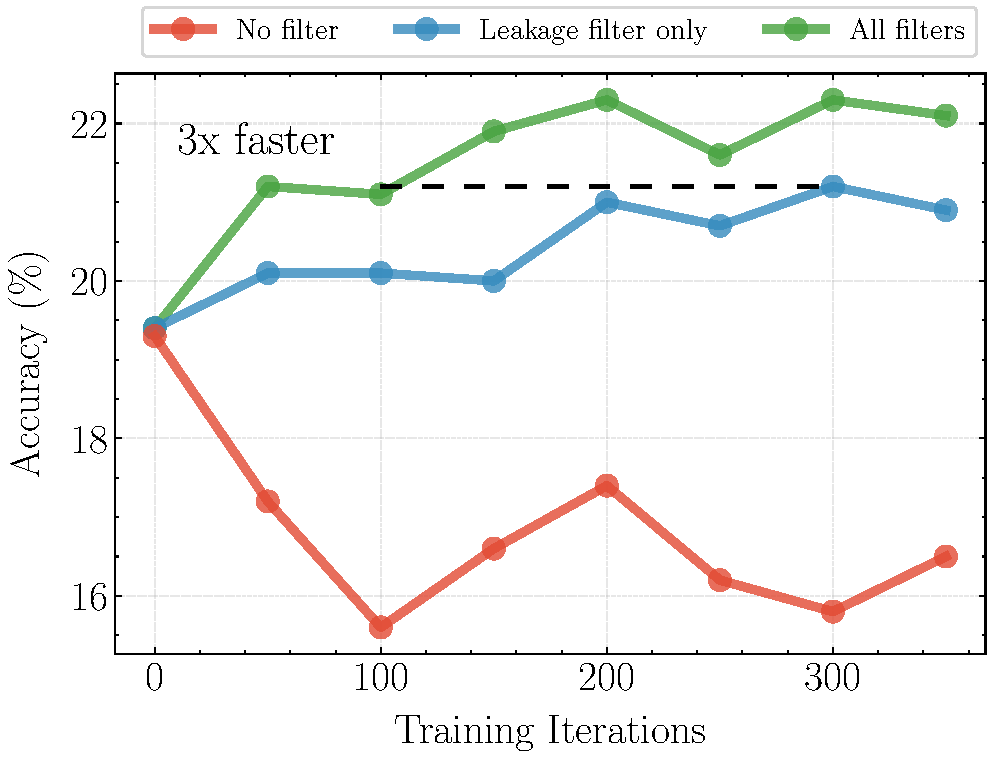
\includegraphics[width=0.95\linewidth]{figures/datafiltering/data_filtering_training_progression_recreated_accuracy.pdf}
\end{minipage}
\hfill
\begin{minipage}{0.48\textwidth}
    \resizebox{\linewidth}{!}{
\begin{tabular}{lc}
\toprule
\textbf{Stage} & \textbf{Number (\%Total)} \\ \midrule
Source Articles & 248,321 \\ \midrule
Question Generation & 744,963 \  (100\%) \\ 
Validation & 295,274 \   (40\%) \\ 
Best Question Selection & 157,260 \   (21\%) \\ 
%With Leakage (Before Edit) & \ 65,815 \quad \ (42\% of 157,260) \\ \midrule
% Leakage (Post Editing) & \ 6,760  \qquad (4.3\% of 157,260) \\ \midrule
Fixing Leakage & 150,500 \   (20\%) \\ 
Answer Type Filtering & \ 62,279  \ \   (8\%) \\
Resolving after 2024-01-01 & \ 52,183  \ \   (7\%) \\ \midrule
\textbf{Final Set} & \ 52,183  \   (7\%)%(25\% of 248,321) 
\\ \bottomrule 
% \textbf{Final usable questions} & \textbf{14,321} & \textbf{28.7\%}* \\ \hline
\end{tabular}}
\end{minipage}
\vspace{-0.2cm}
\caption{(Left) \textbf{Benefits of our filtering stage.} Without leakage removal (red), the model worsens at forecasting, possibly learning shortcuts. With only the leakage removal step (blue), we find that achieving the same performance requires $3\times$ more compute and data. Applying all filtering steps (green) leads to higher accuracy. (Right) Number of questions after each filtering stage.}
\vspace{-0.4cm}
\label{tab:new_combined}
\end{table}

\looseness -1 \textbf{Validation Set.} We use the same recipe to create a validation set of 207 questions using 500 randomly sampled articles from TheGuardian in the month of July 2025. To ensure high-quality, we used \texttt{o4-mini-high}, a much more capable model than DeepSeek-v3, to generate the seed questions. It is $\sim10\times$ costlier, but followed the generation guidelines better, leading to $\sim$ 40\% retention rate (207 final questions out of 500 starting articles).\vspace{0.15cm}

\looseness -1 \contribution{Result 1: Filtering Improves Performance.}  ~\Cref{tab:new_combined} (left) shows the effect of our filtering steps. We train Qwen3-8B using RL with identical hyperparameters on three data variants: (red) 30,000 original generated questions, without any filtering; (blue) 30,000 samples obtained after the question editing step to remove leakage; and (green) 10,000 samples sourced from Forbes and included in \ourdataset. First, we observe the drastic impact of leakage in training. Training without leakage removal (red) worsens the model, perhaps due to shortcut learning. After the leakage removal steps, training improves the model (blue line). Yet, using all filtering stages (green line) leads to both higher accuracy and Brier score, in one-third the data and training steps. \vspace{0.15cm}

In \Cref{sec:binary_ablations}, we also ablate the effect of training on binary-only, free-form-only, and combined binary and free-form data for \texttt{Qwen3-8B}. We find that free-form data is crucial for improving open-ended forecasting, however, training solely on freeform data does not improve performance on binary Metaculus questions. Training with both kind of questions achieves the best trade-off, so we use this for our final training runs presented in \Cref{sec:results}. 

\textbf{Final training dataset.} Across stages, we remove $\sim90\%$ of questions, yielding a training set of 52K samples, each drawn from a unique article. We evaluated Qwen3-32B on this corpus while providing it the source article alongside the generated questions. The model achieves $95\%$ accuracy confirming high validity. We release this training dataset, as {\ourdataset}.

\looseness -1 \contribution{Result 2: Continued Improvements from Scaling Training Data.}  ~\Cref{fig:training_data_performance} shows the effect of scaling training dataset size. For each dataset size, we report test set (described later) results from the best validation checkpoint over prolonged training runs. We use Llama-3.1-8B-Instruct as it starts without any RL post-training. We see continued, and large gains in both accuracy and Brier score as we continue to scale up the training data, demonstrating the importance of our contribution in releasing \ourdataset.


\begin{figure}[t]
\vspace{-0.25cm}
    \centering
    % Legend

    % (a) left plot
    \begin{subfigure}[t]{0.49\textwidth}
        \centering
        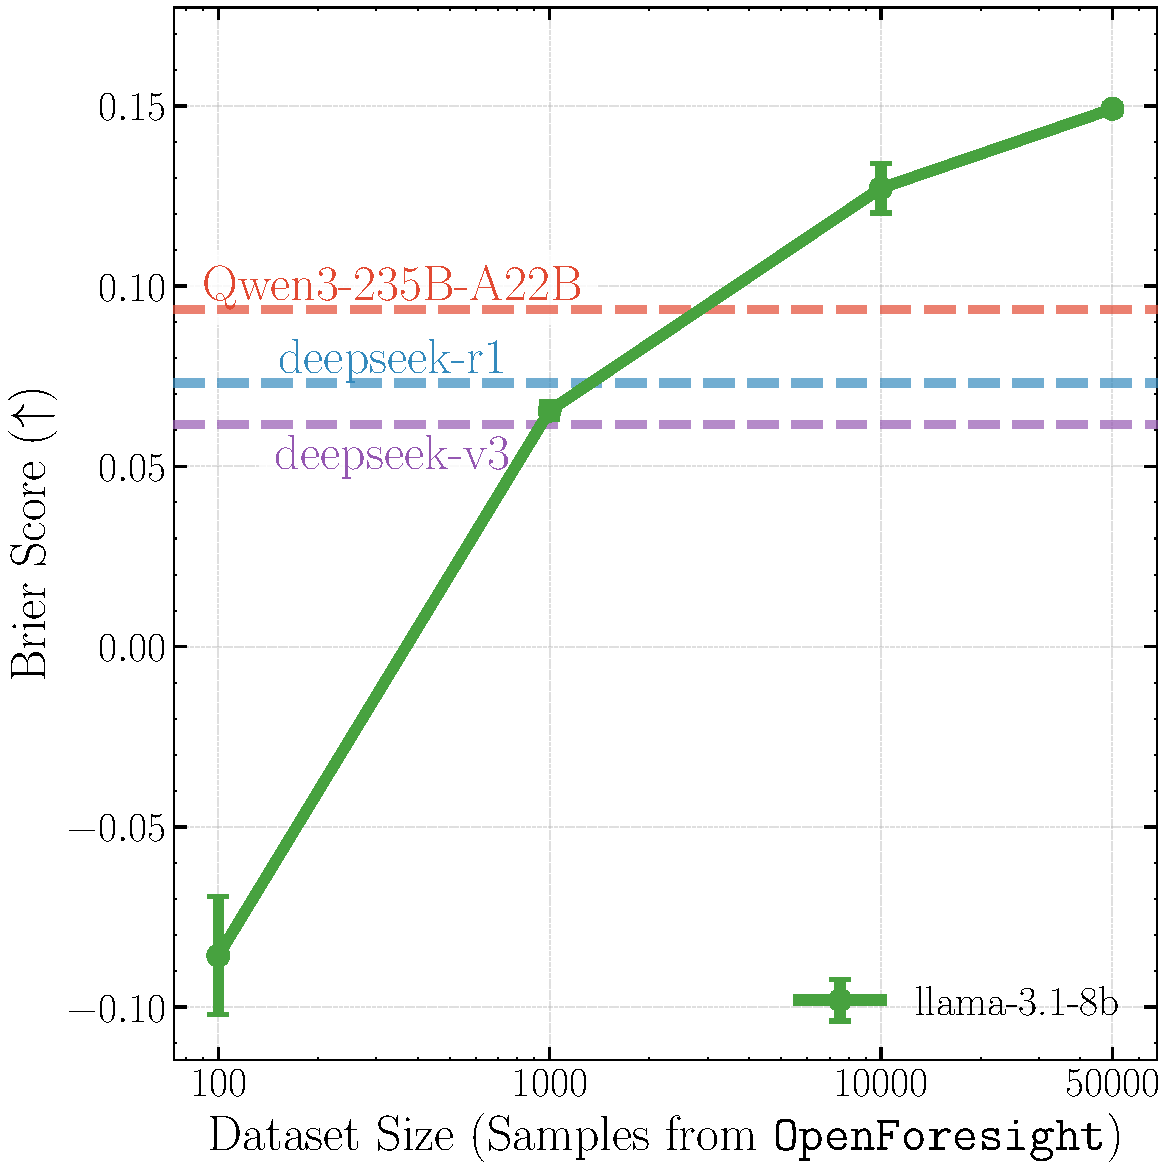
\includegraphics[width=0.9\linewidth]{figures/scaling_data/brier_scores_trainsamples_llama-3.1-8b.pdf}
        % \caption{Performance on our open-ended forecasting test set.}
        \label{fig:training_data_brier}
    \end{subfigure}
    \hfill
    % (b) right plot
    \begin{subfigure}[t]{0.49\textwidth}
        \centering
        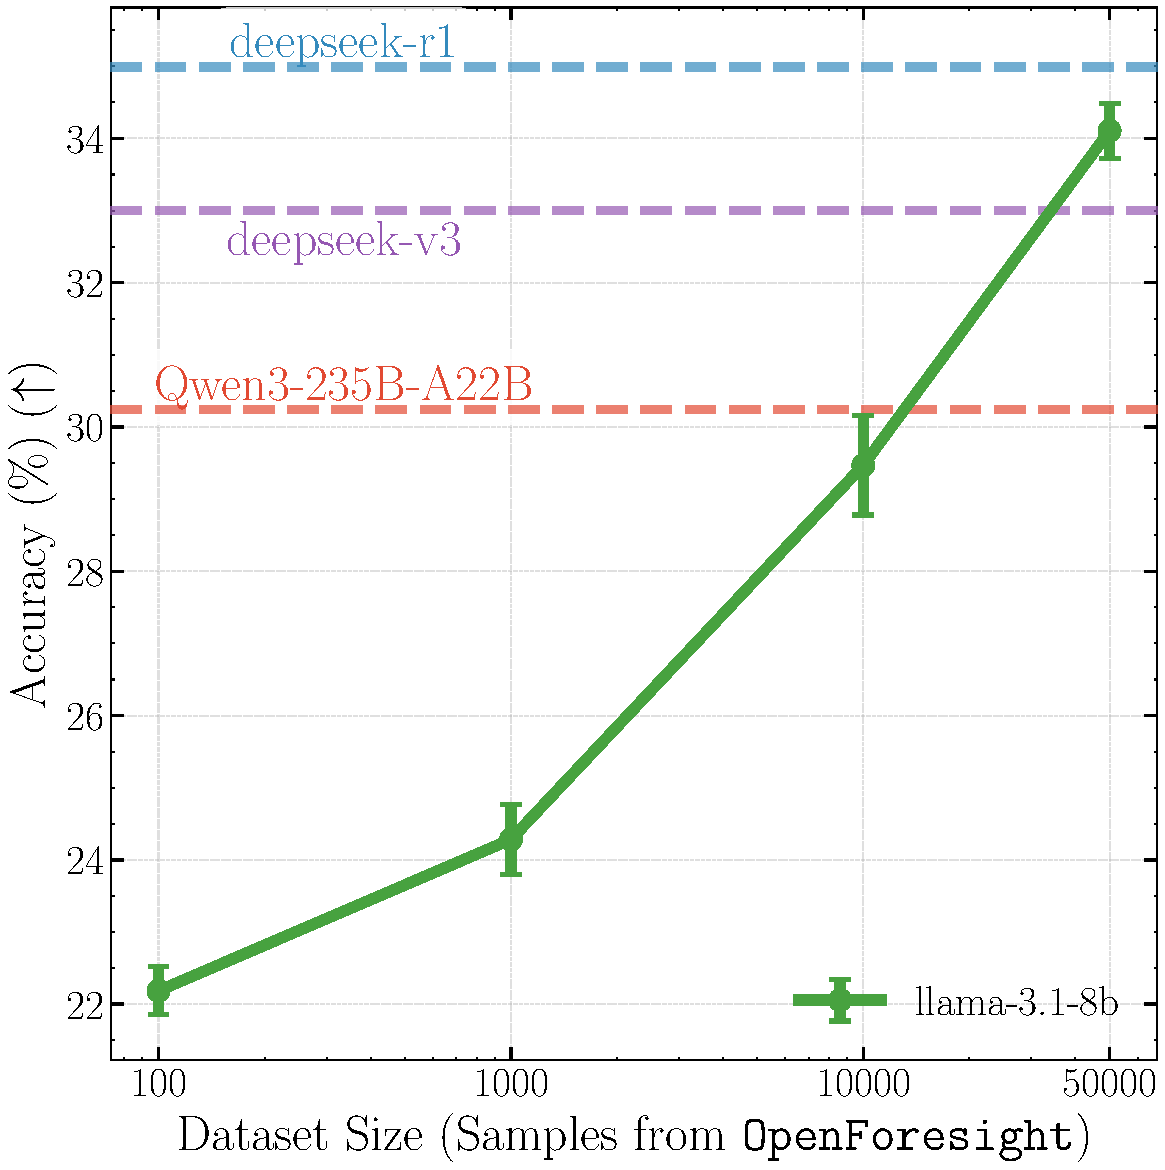
\includegraphics[width=0.9\linewidth]{figures/scaling_data/accuracy_trainsamples_llama-3.1-8b.pdf}
        % \caption{ Performance on the FutureX benchmark. }
        \label{fig:training_data_acc}
    \end{subfigure}

    \caption{
        \textbf{Benefits of scaling training data.} We take the best scores from training Llama-3.1-8B-Instruct on different sized subsets of \ourdataset. We see continued improvements in both accuracy and brier as the data size increases, eventually making Llama-3.1-8B-Instruct match or surpass much larger, more recent models.  
    }
    \vspace{-.4cm}
    \label{fig:training_data_performance}
\end{figure}
